\chapter{Results and Discussion}

This chapter discusses the analysis of the traffic and weather data. Moreover, this chapter will also discuss about the experiments performed and its results to evaluate the analysis of traffic and weather.

\section{Traffic and Weather Analysis}

To be able to extract the relationship between these two independent datasets, we need to understand the underlying pattern of each other and its effect on one another. In this study, we approached this in three steps. First, patterns of traffic and weather are analyzed as independent entities. From this, patterns are compared to identify the relationship between these two entities. Once these patterns are bridged, instances of weather disruption to traffic are derived by associating the weather variables that may be a contributing factor to traffic.





\subsection{Weather Analysis}

\subsubsection{Seasonality}

Seasonality refers to a predictable pattern of a time series data that regularly repeats after a number of intervals. Weather, in the long term, is known to have a yearly pattern such that dry season is expected to occur around November to May, and wet season to occur around June to October. Viewing it in a short-term, meanwhile, it could be observed that they also have a daily pattern as well. For instance, the temperature pattern starts by rising in the morning, peaking in the afternoon, then starts falling in the evening.

	In spite of having a daily pattern, however, there are weather variables whose pattern would not last for every day of the year or even a week. One of these weather variables is precipitation. In the autocorrelation of precipitation (see Figure \ref{figure_autocorr_precip}), it could be observed that despite having a daily seasonality, the pattern of the previous day cannot be barely used to predict the amount of precipitation to be expected today, as indicated by the weak correlation as it approaches its daily seasonality. Comparing it to the autocorrelation of temperature (see Figure \ref{figure_autocorr_temp}), the pattern of the previous day or even until a week ago can be used to predict the incoming temperature of the day, as indicated by the consistently strong correlation throughout the week.


\begin{figure}
  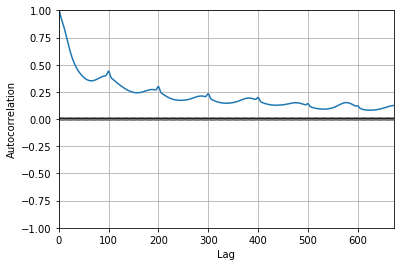
\includegraphics[width=\linewidth]
  {figures/figure_autocorr_precip.png}
  \caption{ Autocorrelation of precipitation showing a loose relationship with its daily seasonality}
  \label{figure_traffic_peakhour}
\end{figure}


\begin{figure}
  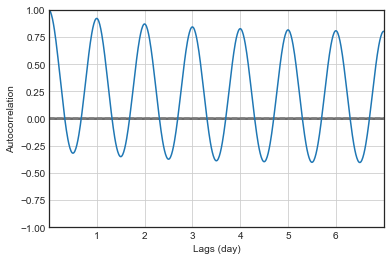
\includegraphics[width=\linewidth]{figures/figure_autocorr_temp.png}
  \caption{Autocorrelation of temperature showing a strong relationship with its daily seasonality}
  \label{figure_traffic_peakhour}
\end{figure}









With these weather variables having a shorter term pattern, these could have situational effects to related or dependent variables whose usual pattern may be disrupted. Thus, we classify these variables as \textit{disruptive variables}. These include wind speed, wind gust, precipitation, and visibility (see Figure \ref{figure_disruptive_var}). Looking at the multicollinearity of these variables (see Figure \ref{figure_weather_corr}), it could be observed most disruptive variables have a strong correlation with precipitation. Particularly, both visibility and wind gust are strongly correlated with precipitation, having a correlation value of -0.787 and 0.600 respectively; and wind gust is strongly correlated with wind speed, with a correlation value of 0.934.


\begin{figure}
  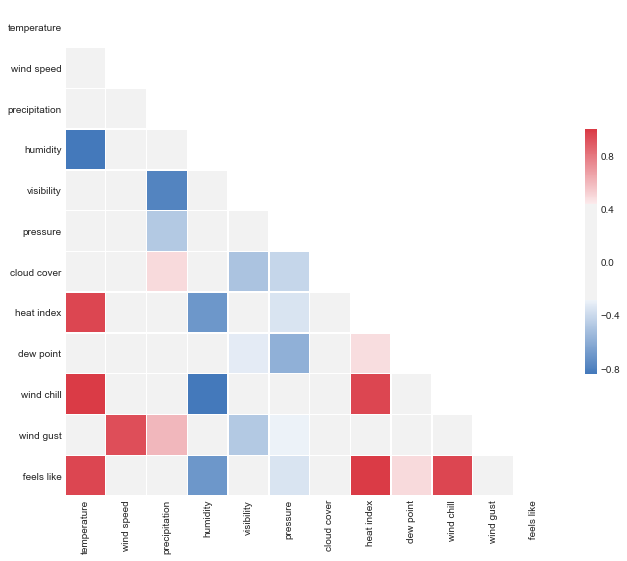
\includegraphics[width=\linewidth]{figures/figure_weather_corr.png}
  \caption{Correlation heatmap of weather variables}
  \label{figure_weather_corr}
\end{figure}








\subsubsection{Trend of Disruptive Variables}

Although these disruptive variables have a shorter term pattern, some still follow certain trends despite being influenced by other disruptive variables. One of which is wind gust (see Figure \ref{figure_windgust}). Similar to non-disruptive variables, wind gust follows a long-term pattern yet is heavily impacted by other disruptive variables, specifically precipitation. It follows the trend of gradually falling until noontime, rising and peaking during the afternoon, and falling at a similar rate during the evening.


\begin{figure}
  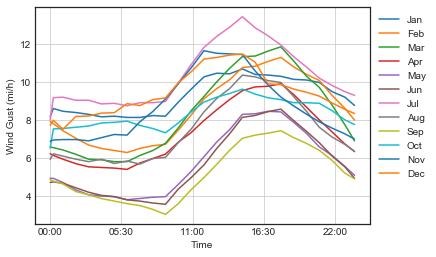
\includegraphics[width=\linewidth]{figures/figure_windgust.png}
  \caption{Daily average of wind gust per month revealing its normal trend despite having a loose daily seasonality}
  \label{figure_windgust}
\end{figure}





In instances where precipitation is abundant, however, there is an immediate effect to its pattern. Figure \ref{figure_precip_temp_windgust} shows a comparison of the impact of precipitation to temperature and wind gust in one of the days under Typhoon Egay. It could be observed that the precipitation did not significantly impact the pattern of the temperature. Nevertheless, we could see how it gradually decreased the temperature from its usual pattern in that specific month. Comparing it with wind gust, it could be observed that the effects of precipitation already took an effect on the pattern of wind gust as it starts to build up. Wind speed, being strongly correlated with wind gust, follows this trend as well (see Figure \ref{figure_precip_windspeed}).



% \begin{figure}
% \begin{subfigure}{0.49\textwidth}
% 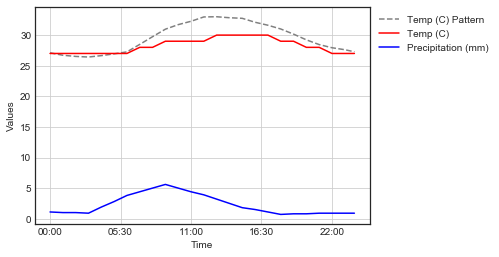
\includegraphics[width=\linewidth]{figures/figure_precip_temp.png}
% \caption{First subfigure} \label{fig:1a}
% \end{subfigure}
% \hspace*{\fill} % separation between the subfigures
% \begin{subfigure}{0.49\textwidth}
% 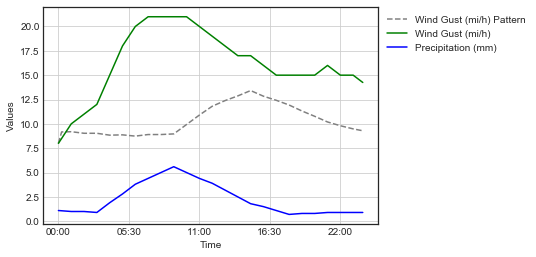
\includegraphics[width=\linewidth]{figures/figure_precip_windgust.png}
% \caption{Second subfigure} \label{fig:1b}
% \end{subfigure}
% \end{subfigure}
% \caption{Comparison of the effects of precipitation to the normal pattern of temperature (a), a non-disruptive variable, and wind gust (b), a disruptive variable} \label{figure_precip_temp_windgust}
% \end{figure}





\begin{figure}
  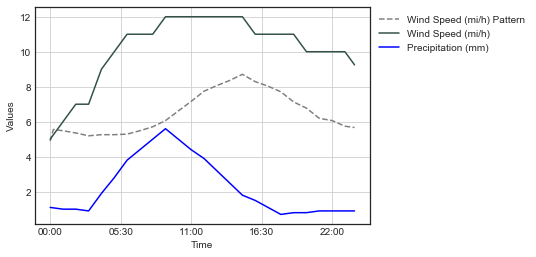
\includegraphics[width=\linewidth]{figures/figure_precip_windspeed.png}
  \caption{Comparison of the effects of precipitation to the normal pattern of wind speed}
  \label{figure_precip_windspeed}
\end{figure}



In a similar way, precipitation also affects other disruptive variables, mainly visibility. Contrary to wind gust and wind speed, visibility does not have a long-term pattern. Rather, it has a strong negative correlation with precipitation, hence its short-term trend is dependent on precipitation instances (see Figure \ref{figure_precip_visibility}).

\begin{figure}
  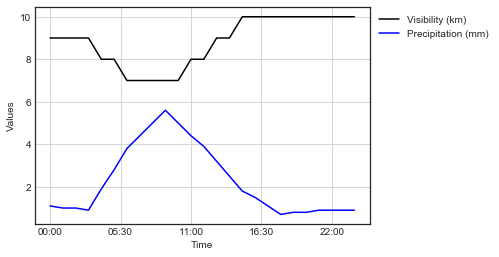
\includegraphics[width=\linewidth]{figures/figure_precip_visibility.png}
  \caption{Negative relationship between visibility and precipitation}
  \label{figure_precip_visibility}
\end{figure}











\subsection{Traffic Analysis Analysis}

\subsubsection{Seasonality}

On an average day, traffic could be linked with the people's daily transportation demand. One example of these is the daily commute of people, attributed to their organizational duties (i.e. 9 to 5 jobs) and academical duties. Built upon these expected demands, the daily seasonality of traffic has been established, following the concept of peak hour. Peak hour refers to the busiest hour where traffic is expected to rapidly rise. In the case of Metro Manila, peak hours are expected to occur from 7 AM to 10 AM, when people leave their home to go to their respective organizations, and 4 PM to 7 PM, when they depart their organizations and return home \cite{metro_manila_peak_hour}.

	However, knowing that there are other contributing factors to traffic, its pattern is not consistent despite its daily seasonality. Analyzing its autocorrelation (see Figure \ref{figure_autocorr_traffic_week}), it could be observed that in spite of its daily pattern, its succeeding days are loosely correlated with the present one. Interestingly, though, the traffic pattern of the previous day could also be used as much as the succeeding days or even the week after. Furthermore, compared with the previous days, it could be observed the present traffic is more correlated with its 7-days-ago pattern or its previous week (e.g. relate the present Monday with last week's Monday).
    
    
\begin{figure}
  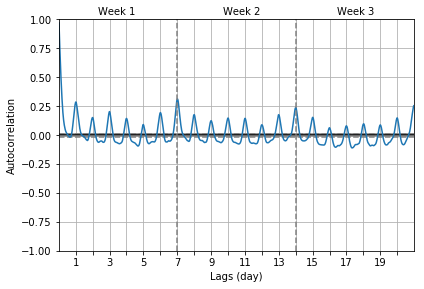
\includegraphics[width=\linewidth]{figures/figure_autocorr_traffic_week.png}
  \caption{Autocorrelation of traffic revealing its daily and weekly seasonality}
  \label{figure_autocorr_traffic_week}
\end{figure}



Viewing its pattern in a longer term, nevertheless, its weekly pattern becomes looser as months go by (see Figure \ref{figure_autocorr_traffic_month}). In other words, it is recommended to expect a certain pattern to last for only four weeks at most. Further examining its seasonality, it could also be observed it does not have a yearly seasonality as well, and its seasonality fades out as time passes by. In simple terms, the traffic pattern in January 2015 is not the same with January 2016. Rather, the traffic pattern in December 2015 is closer to the pattern of January 2016.
    
    
\begin{figure}
  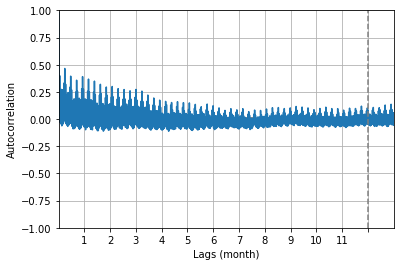
\includegraphics[width=\linewidth]{figures/figure_autocorr_traffic_month.png}
  \caption{Autocorrelation of traffic showing no yearly seasonality}
  \label{figure_autocorr_traffic_month}
\end{figure}


Given these seasonalities, we will explore how traffic changes in its short term and longer term.






\paragraph{Previous Day}

Traffic's daily seasonality could be perceived as causal, such that the traffic of yesterday could be attributed to the traffic of today. For instance, having an intense traffic yesterday morning could be linked with the incoming morning traffic of today. In inheriting the factors of previous days, nonetheless, we also need to take into consideration the concept of working and non-working day.

	A \textit{working day} refers to a day in which people are assigned on duty in an organization  \cite{liu2008wdcm}. For most organizations, it is defined to be on weekdays, Mondays to Fridays, while non-working days are on weekends, Saturdays to Sundays. Aside from weekends, though, non-working days also occur during holidays and government-announced class/work suspension. For our analysis, we treated those days as outliers to our data as the traffic pattern for that particular day is irregular compared with the other weekday working day records. These are important to consider as the transportation demand during working days are higher compared with non-working days \cite{traffic_trend}. For example, the transportation demand of Monday is significantly different from Sunday, thus referencing Sunday for the expected pattern of Monday would be erroneous.

	Comparing the average traffic between working days and non-working days in one month, we could see a significant difference in terms of intensity and pattern (see Figure \ref{figure_workingday_comparison}). Majority of intense traffic occurs at working days. Table \ref{table_traffic_cond_workingday} shows that heavy traffic consists 10.584\% of the working day dataset, while only 0.301\% of the non-working day dataset. Moreover, light traffic consists only 51.819\% of the working day dataset while it accounts for 76.973\% of the non-working day dataset. This, in terms of pattern, indicates that non-working day traffic may follow the peak hour-driven traffic pattern. Therefore, in defining a specific peak hour, we must consider non-working days as an inconsistent case if compared with working days.
    

\begin{figure}
  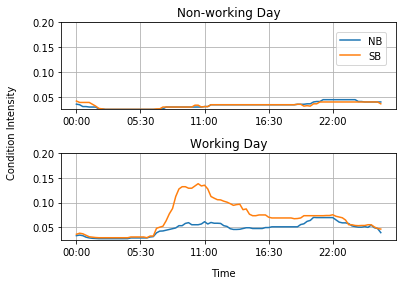
\includegraphics[width=\linewidth]{figures/figure_workingday_comparison.png}
  \caption{Comparison of traffic condition intensity between non-working and working revealing the lack of intense traffic for non-working days}
  \label{figure_workingday_comparison}
\end{figure}

\begin{table}[t]

\centering
\caption{Comparison of traffic condition distribution between working and non-working}
\label{table_traffic_cond_workingday}

\begin{tabular}{|l|r|r|}
\hline
\textbf{Traffic Condition} & \textbf{Working Day} & \textbf{Non-working Day} \\ \hline
L                          & 51.876\%             & 76.973\%                 \\ \hline
ML                         & 4.051\%              & 3.085\%                  \\ \hline
M                          & 31.917\%             & 19.461\%                 \\ \hline
MH                         & 1.573\%              & 0.180\%                  \\ \hline
H                          & 10.584\%             & 0.301\%                  \\ \hline
\end{tabular}
\end{table}


\paragraph{Previous Week}

Traffic could also be related to its week-ago traffic pattern. There has been a concept known as Monday rush hour and Friday rush hour where traffic is expected to increase in the morning and at night respectively. Similar to the previous day approach, we also need to consider working days, but to a lesser degree. Instead, we would only take into account the holidays and suspensions which we will similarly treat as outliers in our reference.


\subsubsection{Rolling and Expanding Features}
The data only describes the traffic condition per time step and the seasonality of traffic. Although the traffic has a pattern, there are instances when a certain disruption in traffic may cause congestion build up. Therefore, considering how the past traffic conditions may affect the current traffic condition may be considered. Although the data from the previous time step can be used as reference in predicting the current traffic condition, the change in traffic in a 15-minute time frame may not be significant. As seen in Figure \ref{figure_workingday_autocorr}, autocorrelation reveals that a traffic condition is highly likely to reoccur every 15 minutes with a correlation value of 0.9918. It does not capture the effects of sudden outliers to the build up or decay of traffic. Thus, it does not fully describe how the past traffic conditions might affect the current traffic condition. 

\begin{figure}
  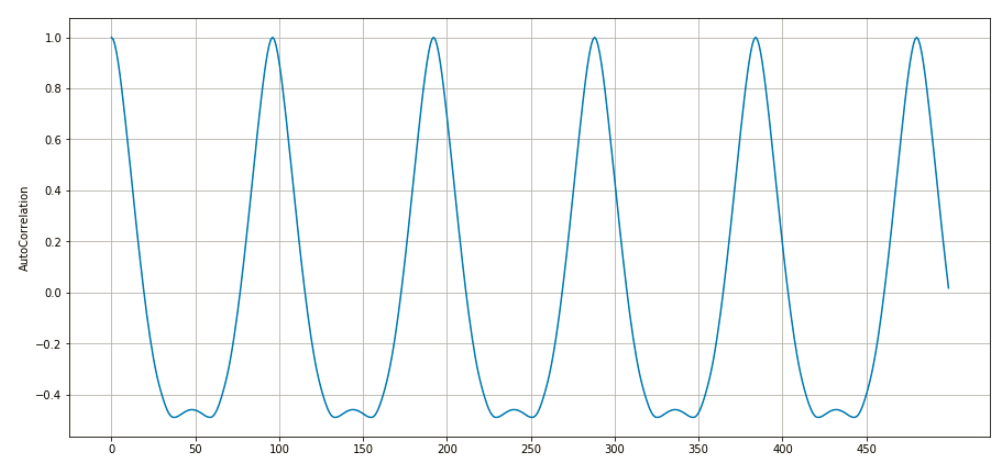
\includegraphics[width=\linewidth]{figures/autocorr_whyRE.PNG}
  \caption{Autocorrelation of traffic for working days}
  \label{figure_workingday_autocorr}
\end{figure}

Generating rolling and expanding features based on a specific window size gives a bigger look as to what the current traffic might be based from the previous traffic conditions. Rolling and expanding traffic features such as the mean, the minimum, and the maximum with window size  4, 8, 24, 48, and 96 were generated from the original traffic data. To summarize the possible effects of sudden changes in traffic, the mean of the past traffic conditions based on a consistent window size was generated. With small window sizes, the values generated captures less of the trifle changes in traffic and gets more affected by outlier values which then results to a more generic information. However, as the window size increases, the effect of outlier values also get more neutralized because of the number of data considered, giving a broader summary of the past traffic. 

Unlike the rolling mean, the expanding mean bases its computations on a growing window size and goes back to 1 when it reaches a specific maximum window size. This lessens the probability of the outlier values getting majorly and consistently neutralized since it always goes back to the original traffic condition from the previous time step. Thus, revealing less generalized details.

The minimum and maximum features, on the other hand, reveals the range of the dataset. Being sensitive to outliers, it allows for outlier detection when compared to the average value of that specific set of data. A big difference between the values of the minimum and the maximum signifies a large progression in traffic condition. Although as the window size used gets bigger, it becomes harder to determine whether the sudden change in traffic condition occurred just a few time steps before or if it is because of a farther instance which may have less to no effect to the current traffic condition. 

Figures  \ref{fig:EspanaRE} and  \ref{fig:RoxasRE} show the average correlation of northbound roads of Espana and southbound roads of Roxas Boulevard per window size in relation to traffic for both rolling and expanding windows. On average, the original traffic has a strong relationship with small rolling windows, specifically window 4 with a correlation value of 0.7501. It is noticeable, however, that the strength of the relationship dwindles down as the rolling window size increases. This reveals that although having a bigger window size means being able to capture various changes in traffic condition, it does not give importance to the most recent traffic conditions. Big changes in traffic conditions that occurred way back and may not have any effect on the current traffic are being considered. Thus, causing its misalignment to the original data. 

In the case of expanding windows, the strength of the relationship to the original traffic also decrease as the window size gets bigger, albeit not so much as the rolling mean do. Looking into both graphs, the strength of the relationship given by window 4 for both rolling and expanding is distinctly stronger compared to  the ones with larger window size. This might be because as mentioned earlier, traffic doesn’t usually change significantly within a small window. As more windows are considered, more and more time steps of traffic data are observed. This will eventually capture some changes in traffic such as outliers and remove them from the generalization. This is shown in Figure \ref{fig:bluementritt_rolling} and \ref{fig:bluementritt_expanding}, where rolling and expanding at window 96 generalizes the high congestion levels into information that is no longer close to reality. Furthermore, the plodding decrease of correlation strength in expanding features as compared to rolling features is caused by limiting the number of windows that the feature grows to and considers and the restarting of its window size. Not limiting the window size growth of expanding features would produce values that are very far away from reality because it would consider every data from the previous days. It would contain values that considers data that are not relevant in predicting the future traffic.

\begin{figure}
  	\centering
    	\captionsetup{justification=centering}
  	\subfloat[Original vs. Rolling]{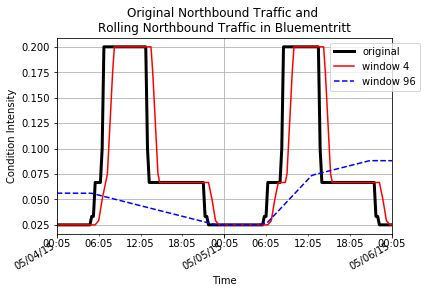
\includegraphics[width=0.5\textwidth]{bluementritt_rolling.png}\label{fig:bluementritt_rolling}}
  	\hfill
  	\subfloat[Original vs. Expanding]{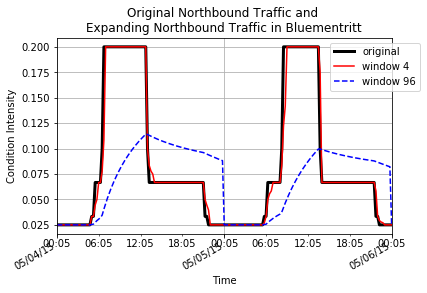
\includegraphics[width=0.5\textwidth]{bluementritt_expanding.png}\label{fig:bluementritt_expanding}}
  	\caption{Comparison of Rolling and Expanding windows 4 and 96 to original Southbound traffic in Bluementritt}
\end{figure}

\begin{figure}
  	\centering
    	\captionsetup{justification=centering}
  	\subfloat[EspanaRE]{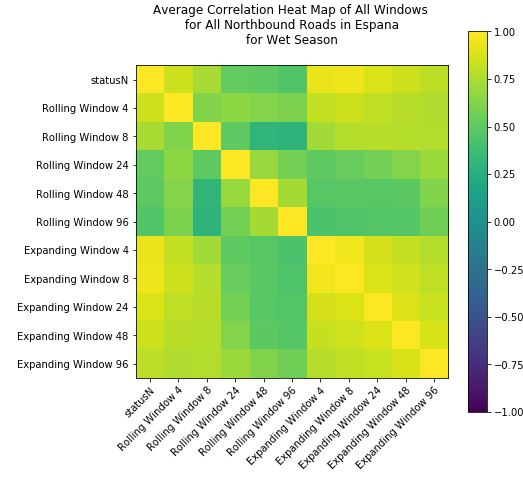
\includegraphics[width=0.5\textwidth]{figures/heatmap_espana.JPG}\label{fig:EspanaRE}}
  	\hfill
  	\subfloat[RoxasRE]{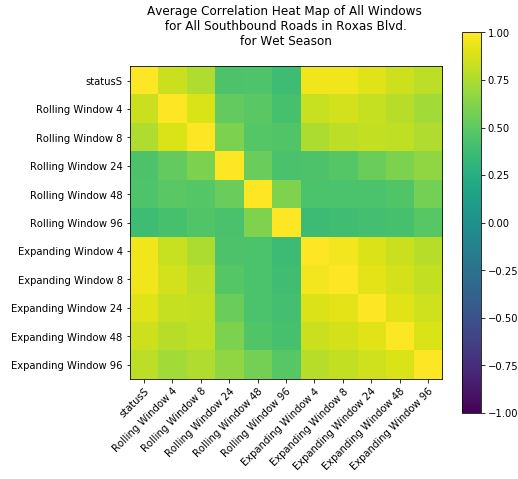
\includegraphics[width=0.5\textwidth]{figures/heatmap_roxas.JPG}\label{fig:RoxasRE}}
  	\caption{Average Correlation of Rolling and Expanding Features for Espana and Roxas Blvd.}
\end{figure}
